\documentclass{article}
\usepackage{graphicx}
\usepackage[ampersand]{easylist}
\usepackage{fullpage}
\usepackage{url}

\begin{document}

\title{Deliverables Summary}
\author{Michael McDonnell}

\maketitle
\section*{Introduction}

The thesis focus for the year was attempting to develop a system to allow a self driving vehicle to identify road features to set the conditions for navigation through features such as intersections.

The development attempted to follow an AGILE approach with iterative increases in functionality. A simulation system was developed to provide camera feed inputs to a Python process. The core deliverables discussed were:
\begin{easylist}[itemize]
	& \textbf{Journal or Conference paper.}
	& \textbf{Simulation with Inter Process Communication.}
	& \textbf{Navigation localisation system.}
\end{easylist}

During the course of development familiarity was gained in a range of additional areas. Edge detection was investigated as an initial road detection attempt and the use of convolutional neural networks was investigated as an alternate option. As a result of this work outside the core system, the following additional deliverables have been developed:
\begin{easylist}[itemize]
	& \textbf{MATLAB assignment resources for Computational Problem Solving.} 
	& \textbf{Sprint review example.} 
	& \textbf{Machine learning familiarisation activities}
\end{easylist}



\section{Journal or Conference Paper}

It was identified that \textit{Robotics and Autonomous Systems} is a suitable journal to submit a paper to. This journal deals with the core subject material, has an impact factor of 2.928 and has a clearly detailed submission process. If the paper is not accepted into this journal alternative options will be considered including conferences including optimistically, the 17th International Conference on Ubiquitous Robots (UR 2020) - Kyoto with a submission date of early 2020. A more flexible option is one of the various International Conferences on Control, Automation, Robotics and Vision Engineering throughout 2020.

The initial draft is aligned to the Robotics and Autonomous systems general format however content, style and length can be massaged based on submission target.

\section{Simulation with Inter Process Communication}

A lightweight simulation was developed to assist in data generation for the development of the navigation localisation system for the thesis. This system presented significant challenges in developing a method to communicate sensor data from the simulation to the Python process. Inter Process Communication (IPC) was implemented with ZeroMQ which allowed communication between Unity (C\#) and Python. 

As the system developed it was found the only information needed from the Unity simulation was the camera image feed so the IPC setup was developed around this specific need however a more advanced communications architecture was planned. While this was not implemented, the logic behind it was preserved and is included with the simulation documentation. 

The simulation itself contains a simple waypoint following AI and basic sensors. It provided effective data for the system being developed for the thesis but also represents a starting point for a more advanced and generic simulation. Included files are:

\begin{easylist}
	& The Unity project for the simulation (\textbf{VehicleSimluation} folder)
	& \textbf{PythonZMQServer.py} - The Python script required for the IPC server.
	& The simulation system documentation including an overview of the Unity project, IPC communications and the planned architecture for a more advanced communications protocol between an external process and the simulation.
\end{easylist}

\section{Navigation localisation system}

The provided system includes test data for a proof of concept. In addition to the provided files, \textbf{cv2} and \textbf{numpy} are both required. Provided files are as follows:

\begin{easylist}[itemize]
	& \textit{nav\_localisation.py -} This is the core file which is run. The default method here calls a single \textit{main} method and passes test data (see below). The main work in this script is from the \textit{process\_frame} method which maintains a simple state using boolean flags to determine if detection or tracking code is run. This script also contains visualisation code as well as video saving function.
	& \textit{road\_surface\_detection.py -} Class to use as a road detector, implements Histogram backprojection road surface detection. \textit{get\_road\_surface\_from\_new\_frame} is the Class method called to detect the road surface in a new frame.
	& \textit{feature\_tracker.py -} Obtain initial feature mask using \textit{get\_feature\_masks} and check for feature detection using \textit{check\_feature}. This includes argument for optical flow which is estimated using \textit{GetUpdatedRoadFeatureLocationFarneback}.
	& \textit{bezier.py -} Helper script to develop bezier curve mask using \textit{get\_curve\_mask}. Generic in that \textit{draw\_bezier} can be called directly to draw bezier curve to any image.
	& \textit{test\_data.py -} Implements the data interface required (see following subsection) and contains test methods to confirm data.
\end{easylist}


\subsection{Data interface}

The system expects a data interface with the following methods:

\begin{easylist}[itemize]
	& \textit{get\_next\_feature() -} Returns next feature or None if no more available.
	& \textit{get\_next\_frame() -}	Returns next image frame (either from video stream or saved images).
	& \textit{get\_inverse\_perspective\_matrix() -} Returns the inverse perspective matrix developed for this dataset.
	& \textit{get\_ipm\_mask() -} Returns a mask which defines the area of information for the inverse perspective matrix.
\end{easylist}

The provided code demonstrates the concept of the system and is suitable for extension, generalisation and improvement. Any script that implements the data interface can be passed to the main method in \textit{nav\_localisation.py} for processing which allows easy implementation of multiple different input source files. The data interface provided uses images and an inverse perspective transformation matrix included in the \textit{TestData} subfolder. 


\section{MATLAB assignment resources for Computational Problem Solving}

It was identified that filter convolution is a (relatively) simple algorithm to implement and may be a suitable teaching case for a practical implementation of loops. In lieu of developing a specific assignment, a set of relatively simple set of convolution operations using functions over several files is included as a starting point for an assignment.

The files include operations on two images using a combination of smoothing (blur) and median filters as well as edge hardening (subtracting smoothed image from original image) and masking. These algorithms have been implemented naively using nested loops with helper functions to ensure the logic is as clear as possible. Helper functions include getting a filtered value (filtering a single point involves two nested loops) and a `safe getter' which will return a value or 0 if a coordinate is out of bounds.

\begin{easylist}[itemize]
	& \textbf{Images.mat} - MATLAB variable file with both images saved.
	& \textbf{ProcessImages.m} - Base file to run to demonstrate operations on both images. Assuming data has been loaded from \textbf{Images.mat}, the following files can be run for individual demonstrations:
	&& \textbf{FarmImage.m}
	&& \textbf{CountrysideImage.m}

	& Core files:
	&& \textbf{RunFilter.m} - Apply a convolution filter to an image using nested for loops. 
	&& \textbf{MedianFilter.m} - Apply a median filter to an image. Median filter sets the new pixel value to the median value over the filter size about the point. This is very useful for the removal of 'salt and pepper' noise.
	
	& Helper files:
	&& \textbf{ValueFromFilterCoord.m} - Get a single convolution value for a pixel. This function applies the convolution filter about a location on the image defined by an x, y coordinate.
	&& \textbf{Threshold.m} - Simple thresholding function implemented as nested loops with conditionals. Thresholding returns a binary image (black and white) where pixels of value greater than the threshold will be white and lower than a threshold will be black.
	&& \textbf{NormaliseImage.m} - Helper function to normalise an image from 8 bit to floating point between 0 and 1.
	&& \textbf{MedianFromCoord.m} - Helper function to return the median value within a provided filter size (x and y) about a point. 
	&& \textbf{GetValueOrZero.m} - Helper function to 'safely get' a value within a matrix. If the provided coordinates fall outside the matrix dimensions, return 0 instead.
	&& \textbf{MaskFilter.m} - Helper function to mask out all elements of an image outside a provided rectangle bounds.
\end{easylist}

These files represent a verbose loop based implementation of simple image processing. A possible assignment task is to provide these files with portions and/or full implementations missing. As an example the core files could be provided without the loops implemented and files such as \textbf{GetValueOrZero.m} could be provided without any implementation code to be filled out. The exact task is dependant on the level of expected competency of students. Extensions to this task could involve improving the implementation, for example the \textbf{conv2} function (\url{https://au.mathworks.com/help/matlab/ref/conv2.html}) can replace the majority of core and helper files. Providing a hint that 2D convolution is the task they are undertaking would allow exercising of documentation research (while being simple enough that googling `MATLAB 2d convolution' would lead to the answer).

\section{Sprint review example.}

The feature development of the system and simulation was managed using an AGILE approach. This involved incremental feature delivery with a fortnightly review. Fortnightly reviews included triaging of future work but also the provision of an update to interested stakeholders. The review includes the `velocity' over the previous fortnight which is a quantified measure of work based off the estimated `story points' per task that were completed in the sprint. Following this a presentation of the current capability (generally focussing on impactful demonstrations of new features developed) occurs and discussion with stakeholders. After the sprint review, tasks are selected for work over the following fortnight based off the existing velocity. This assists with planning time allocations (using existing knowledge to estimate small task difficulty) while retaining flexibility to rapidly pivot in focus.

The sprint reviews throughout the year morphed into an informal brief review due to the difficulty in locking in standing appointments however the theory was maintained. An example of a formal sprint review is included as an example to individuals in future that may be interested in adopting this approach and are looking for a starting point.

\section{Machine learning familiarisation activities}

The use of Convolutional Neural Networks (CNN) for road surface detection was considered during the thesis. As part of analysing the potential effectiveness of this solution an effort was made to develop a robust understanding of neural network (and more generally, machine learning algorithms) implementation from first principles as well as small `toy' projects to gain a working familiarity with implementation details. A focus on interpretable AI and a desire to have a more complete solution (with driving lines and intersection tracking) meant that a CNN approach was not pursued however a good understanding of the application was developed.

Three elements are presented here to highlight the work undertaken regarding machine learning familiarisation.

\subsection{Machine Learning course}

The Stanford University online Machine Learning course was undertaken through Coursera (\url{https://www.coursera.org/learn/machine-learning}) which provided a mathematical understanding of multiple machine learning algorithms. The course is delivered by Andrew Ng \footnote{Andrew NG credentials include: CEO/Founder Landing AI; Co-founder, Coursera; Adjunct Professor, Stanford University; formerly Chief Scientist,Baidu and founding lead of Google Brain} over 11 weeks and includes the mathematics and development from first principles in MATLAB of multivariate linear regression, logistic regression, regularisation, neural networks (forward and backpropogation), Support Vector Machines, k-Means and Principal Components Analysis. The course culminates with examples (and implementation from first principles) of anomaly detection, recommender systems and a simple optical character recognition. This course was completed with 100\% over all quizzes and code assignments. The certificate of completion of this is included. 

On completion of this course familiarisation projects were developed using Python and Keras which is a Tensorflow wrapper. Two of these projects which may be candidates for extension for future student projects are discussed in the following subsections.


\subsection{Where's Wally Solver - Neural Network with sliding window (Unsuccessful)}

The first familiarisation attempt for Convolutional Neural Networks in Keras was to develop a system to find Wally in the Where's Wally puzzles. While this was ultimately unsuccessful, I believe the final approach had promise and may work better with both more robust training data (likely through data augmentation) and optimisation of network topology. 

Initial approaches involved attempting to `brute force' the learning by feeding multiple images in with the normalised coordinates of Wally's face. This was not successful and a more refined approach was developed. This involved the use of dynamic resolution scaling sliding windows; in lieu of looking for Wally in the full image, a window of interest (initially the full window) is resized to the network input dimensions and run through a binary classifier which has been trained on images of just Wally's face. This region of interest `slides' over the image and when the full image has been checked, the window of interest size is reduced. The process continues iteratively with smaller and smaller window sizes until a minimum size is reached. The benefits of this approach are likely to be:

\begin{easylist}[itemize]
	& The task being solved by the network is significantly simpler; the network is just a binary classifier which detects if an image contains Wally. The training data consists of `full face' images where Wally takes up most of the image so multiple features can be matched. 
	& The iterative size reduction of the sliding window allows the full image to be considered at different sizes. This means that regardless of how big Wally is in the image, assuming the window scaling factor is correct, there will eventually be a point where a window of an appropriate size is located over Wally such that he fills a significant portion of it.
\end{easylist}

In addition to the training data, a trained model (\textbf{wally\_model.h5}) is included (which does not perform well!) and the following files:

\begin{easylist}[itemize]
	& \textbf{find\_wally.py} - The initial basic implementation which calls the sliding window prediction.
	& \textbf{sliding\_window.py} - Function which manages sliding window implementation including strides and scaling as well as visualisation. The main function called in this is \textbf{do\_all\_roi} which accepts \textit{process\_roi\_func} as an argument which is the function called to process a region of interest. In the \textbf{find\_wally.py} implementation, the trained network prediction function is included here.
	& \textbf{wally\_nn.py} - Interfacing with the trained classifier. Includes test method to run standalone.
	& \textbf{wally\_nn\_setup.py} - The initial training of the binary classifier.
\end{easylist}

%	\begin{figure}
%		\centering
%		\includegraphics[width=3.0in]{myfigure}
%		\caption{Simulation Results}
%		\label{simulationfigure}
%	\end{figure}

To reiterate, while the logic seems sound, the trained model did not perform well and this is not effective as a project however it may provide a starting point for further development. Files for this are included in the \textbf{Wally} subfolder.

\subsection{Symbol recognition - Classification of user input symbols (Successful)}

\textbf{Background.} The motivation for this exercise was real time arbitrary symbol recognition such as may be found in a game where the player `casts' spells by drawing the symbol with a mouse. A minimal Unity project was developed which allowed the rapid generation of training data. The player holds down a button to commence the `cast' and draws a symbol with the mouse. The data generated by this is a binary image with pixel locations drawn over locations the mouse was moved over. This is sampled each frame so the faster the mouse is moved, the further apart individual pixels will be. The point the user commences is marked by a larger `blob' which assists in differentiating between similar symbols with different directions (although the relative pixel spacing differences based on input movement speed may also provide enough information to differentiate these). The Unity project is provided in the \textbf{SpellGesture} subfolder and includes all the functionality required to generate training data based off mouse button presses with the logic fully enclosed in \textbf{SpellCasting.cs}. \\

\textbf{Approach.} Three symbols were developed as allowable options; an E (capital epsilon starting from top right) and two V shapes, one starting either side. These are visualised (along with an incorrect symbol due to Epsilon starting in the bottom right) in figure \ref{symbolPrediction}. This figure represents the correct predictions made by the trained 'Spell Gesture' network.

\begin{figure}[h!]
	\centering
	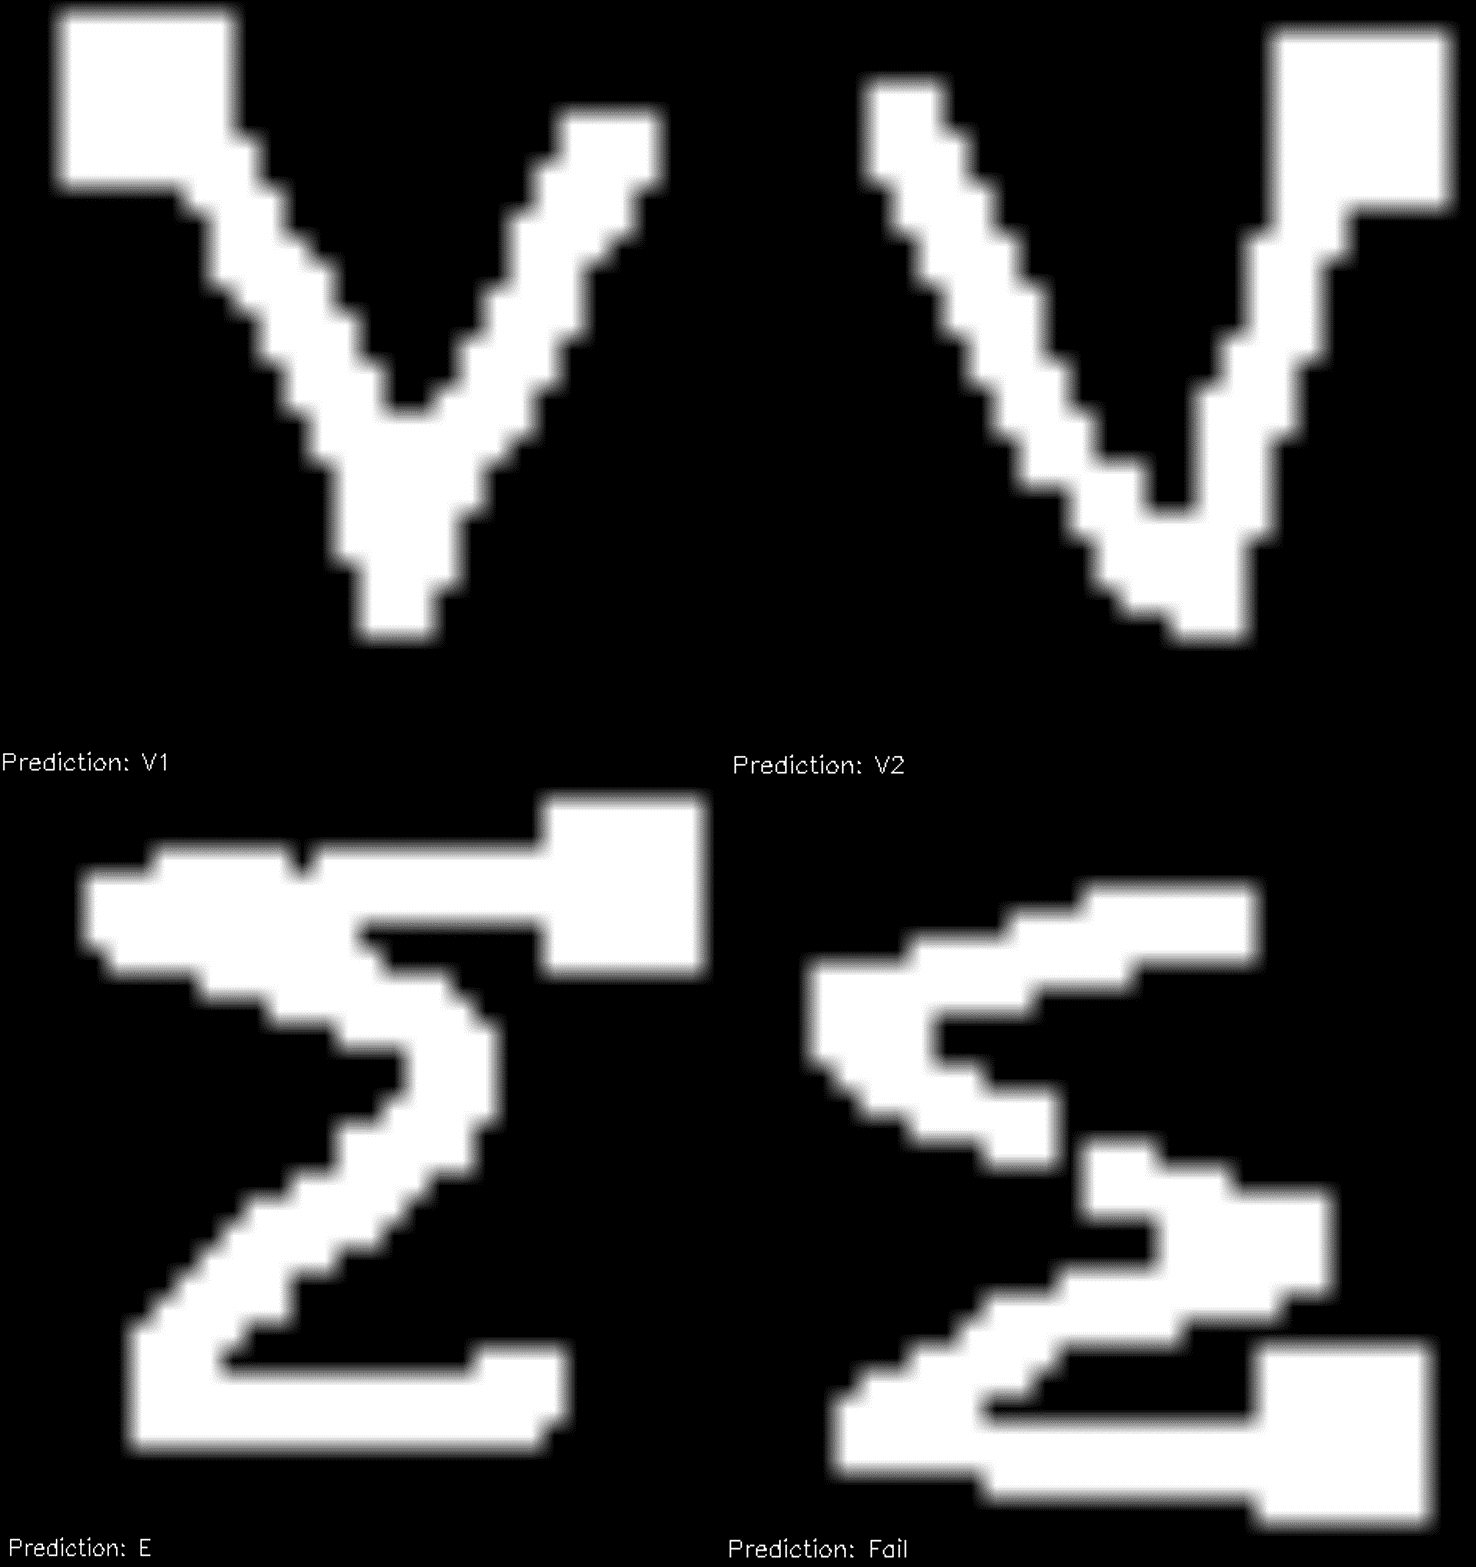
\includegraphics[width=0.5\linewidth]{symbolPrediction.png}
	\caption{Prediction of symbols by `Spell Gesture' network showing two acceptable V variants (top), an acceptable Epsilon variant (bottom left) and a fail (bottom right) due to starting an Epsilon at the wrong location.}
	\label{symbolPrediction}
\end{figure}

The first attempt was to define a 3 output network with [V1, V2, E] as the outputs (where a fail is all zero). This did not work very well as the network seemed biased towards higher values as failures were still being predicted as one of the 3 options. I tried adding a fourth output and set all the fail examples to the first value (ie output = [fail, V1, V2, E] ) and that worked quite well, including correctly classifying the E symbol as a fail when it started at the bottom instead of the top. 

The final approach reverted to the original [V1, V2, E] however the final activation function was changed from softmax to sigmoid. This was an error initially; softmax provides a best guess out of all options; the final output values are normalised to sum to 1. This is why adding a fourth `fail' option (effectively became a catch-all for everything else) performed better. Using raw sigmoid is a much better option when you do not \textbf{need} one of the options to be true. \\

\textbf{Analysis.} Looking at the first tensorboard output (convolutional dropout at 25\%) below it seems that there is an overfitting issue. This was addressed by increasing the dropout to 50\% which generalises the model more (dropout randomly removes connections in training to ensure general patterns are developed as opposed to specific `learned' patterns).

\begin{figure}[h!]
	\centering
	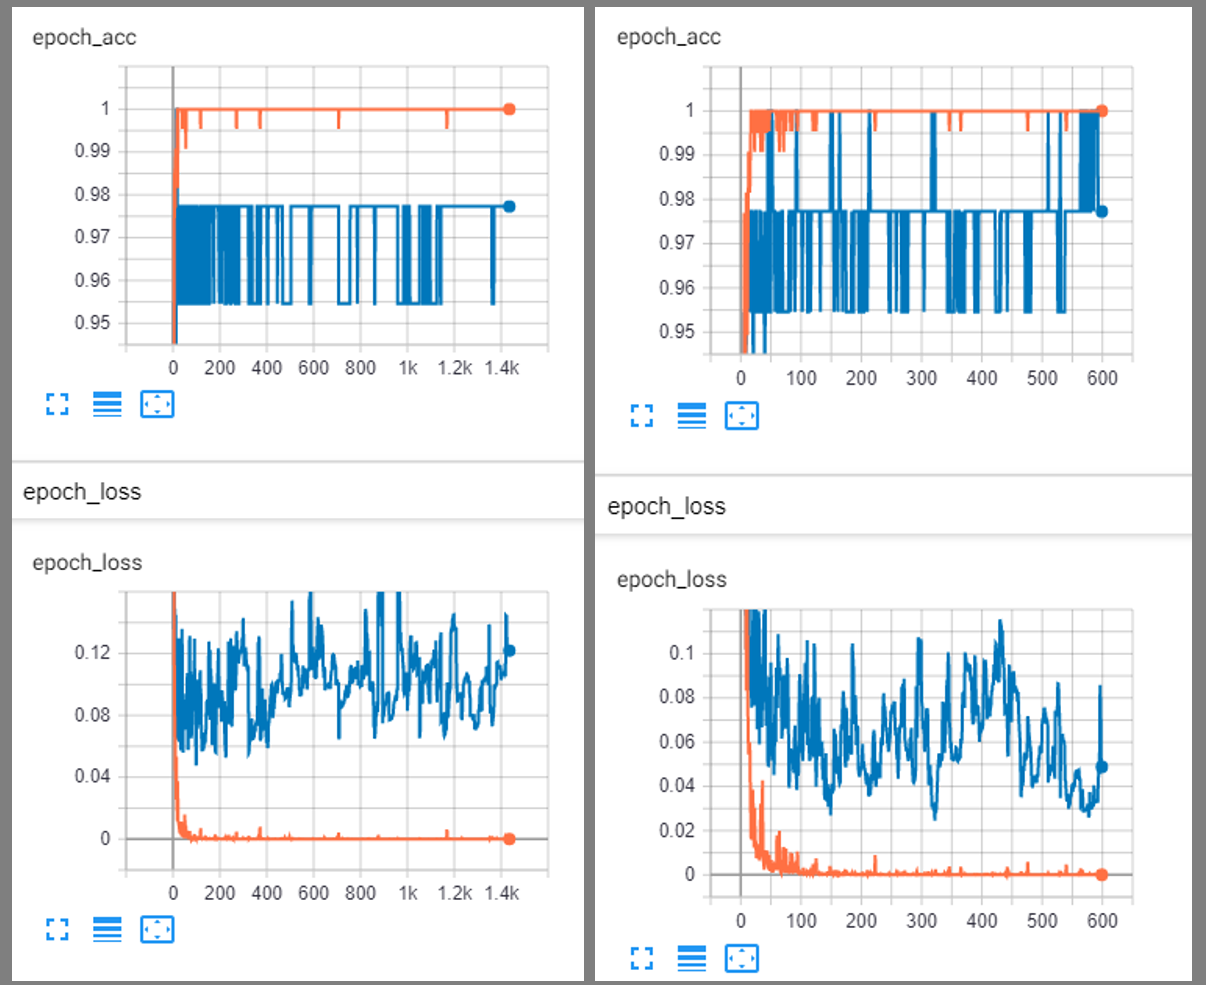
\includegraphics[width=0.5\linewidth]{symbolPerformance.png}
	\caption{Tensorboard visualised performance of `Spell Gesture' network with 25\% convolutional dropout (left) and 50\% convolutional dropout (right)}
	\label{symbolPerformance}
\end{figure}


Training time for the network was negligible (1-2 minutes using GPU for 1500 epochs) and the results (off realistically quite a small training set, even without using the keras image augmentation) were very solid after only ~200 epochs (~20s).\\ 

\textbf{Provided code.} The python code is provided in the subfolder \textbf{SpellGestureCNN} and is relatively straight forward. In addition to the training data and trained models (*.h5 files) the three code files are:

\begin{easylist}[itemize]
	& \textbf{check\_spells.py} - Predicts the value of images in test image folder. \textbf{NOTE:} The model is loaded from an \textit{absolute} path in this file so the correct path will need to be placed in here.
	& \textbf{train\_spells.py} - Creates and trains model on the provided training data. Again paths here are absolute so will need to be modified. Tensorboard callbacks are included here.
	& \textbf{load\_data.py} - Loads all data and sets the category for training data.\\
\end{easylist}

The files for this project are included in the \textbf{SymbolDetection} subfolder.

\section*{Final words}
The project this year was ambitious, challenging and allowed development of conceptual understanding over a range of topics. In addition to the core academic deliverable requirements it is hoped that some of the additional delivered elements may assist others in delving deeper into some of these topics and potentially serve as inspiration for interesting and challenging future thesis or CDF project works. 

\end{document}